\section{Theorie}
Im diesem Versuch wird der RLC-Schwingkreis untersucht, dieser besteht aus folgenden
Bauteilen: Widerstand $R$, Induktivität $L$ und Kondensator $C$.
Ähnlich zum RLC-Schingkreis ist der RC-Schwingkreis aufgebaut, er bestitzt nur einen
Energiespeicher, den Kondensator $C$. Daher kann der Strom $I$ nur in eine Richtung fließen.
Der RLC-Schwingkreis besitzt zwei Energiespeicher, einen Kondensator und eine
Spule. Wird nun Energie in das System hineingpumt pendelt diese zwischen Kondensator und
Spule, wodurch der Strom sein Vorzeichen ändert. Der Widerstand, der hier dem
Dämpfungsfaktor entspricht, wandelt einen Teil der Energie in Wärme um. Nach einer
gewissen Zeitspanne ist keine elektrische Energie mehr vorhangen und die Schwingung
kommt zum erliegen. Dieses Verhalten wirdauch als gedämpfte schwingung bezeichnet.
Wenn kein Widerstand $R$ im System verbaut ist, wird dieses System als
ungedämpften Schwingung bezeichnet.
\begin{figure}[H]
  \centering
  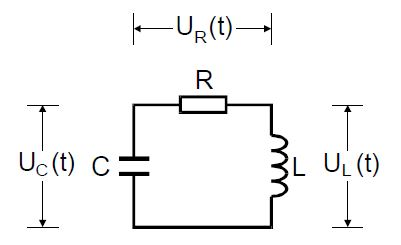
\includegraphics[height=5cm]{RLC.JPG}
  \caption{Darstellung eines RLC-Scwingkreises}
  \cite{skript}.
  \label{fig:RLC}
\end{figure}
Wird an den Schwingkreis von außen eine Spannung angelegt, schwingt dieser
mit der Frequenz der angelegten Spannung. Die so erhaltene Schwingung wird als
ezwungene Schwingung bezeichnet. Hat die von außen angelete Spannung die "richtige"
Frequenz (abhänging vom verwendeten System/Schwingkreis), dann erreicht die Spromamplitude im
Schwingkreis ihr Maximum. Dieser Fall wird als Resomanzfall bezeichnet und tritt bei der
sogenannten Resonanzfrequenz auf.

\subsection{Gedämpfte Schwingung}
In einem RLC-Schwingkreis,der wie in Abbildung \ref{fig:RLC} aufgebaut ist, gilt nach dem
2. Kirchfoffschen Gesetz:
\begin{equation}
  U_{R}(t)+U_{L}(t)+U_{C}(t)=0.
  \label{eqn:max}
\end{equation}
Die Spannungen lassen sich auch wie folgt ausdrücken:
\begin{align}
  U_{R}&=RI\\
  U_{C}&=\frac{Q(t)}{C}\\
  U_{L}&=L\frac{dI}{dt}\\
\text{außerdem gilt:}\:\:I&=\frac{dQ}{dt}.
\end{align}
Eingesetzt in Gleichung \ref{eqn:max} und ableiten nach der Zeit liefert dann die Differentialgleichung
für die gedämpfte Schwingung
\begin{equation}
  \ddot{I}+\frac{R}{L}\dot{I}+\frac{1}{LC}I=0.
  \label{dgl}
\end{equation}
Zur Lösung dieser DGL wird folgender e-Ansatz verwendet: $I(t)=A\exp{i \omega t}$.
Eingesetzt in Gleichung \ref{dgl} ergibt sich
\begin{equation}
  (\omega)^2 -i\frac{R}{L}\omega -\frac{1}{LC}=0
  \label{dgll}
\end{equation}
Umgestellr nach $\omega$ egibt sich daraus:
\begin{equation}
  \omega_{1,2}=
\end{equation}

\subsection{Erzwungene Schwingung}
Nun wird an den gedämpften Schwingkreis eine Spannungsquelle angeschlossen, die
eine Sinusförmige Wechselspannung $U_{S}=U_{0}\exp{i\omega t}$ liefert.
\begin{figure}[H]
  \centering
  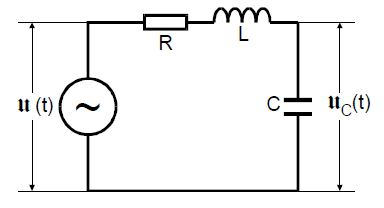
\includegraphics[height=5cm]{erzw.JPG}
  \caption{Schwingkreis mit äußerer Spannungsquelle}
  \cite{skript}.
  \label{fig:erzw}
\end{figure}
Die Differentialgleichung \ref{eqn:dgl} wird nun zu einer inhomogenen DGL der Form
\begin{equation}
  \ddot{I}+\frac{R}{L}\dot{I}+\frac{1}{LC}I=U_{0}\exp{i\omega t}
  \label{eqn:erzwdgl}
\end{equation}






\label{sec:Theorie}

%\cite{sample}
